\documentclass[12pt]{article}
\usepackage[spanish]{babel}
\usepackage[a4paper, margin=1in]{geometry}
\usepackage{times}
\usepackage{setspace}
\linespread{1.5}
\usepackage{graphicx}
\graphicspath{{images/}}
\usepackage[nottoc]{tocbibind}
\usepackage[colorlinks=true, linkcolor=black, citecolor=black, urlcolor=black]{hyperref}
\usepackage{tabularx}
\usepackage[table]{xcolor}
\usepackage{amssymb}
\usepackage{placeins}
% NOTE - Eliminar cuando ya no uses lorem ipsum
\usepackage{lipsum}

% Formato de sangrías y listas
\usepackage{enumitem}
\renewcommand{\labelitemi}{$\bullet$}
\setlength{\parindent}{0.3in}
\setlist[itemize,1]{leftmargin=0.45in}
\setlist[itemize]{leftmargin=0.2in}

% Formato de la tabla de contenido
\usepackage{tocloft}
\setlocalecaption{spanish}{contents}{Índice de Contenido}
\renewcommand{\cfttoctitlefont}{\hfill\normalsize\bfseries}
\renewcommand{\cftaftertoctitle}{\hfill}
\renewcommand{\cftsecleader}{\cftdotfill{\cftdotsep}}
\setlength{\cftbeforesecskip}{0pt}
\setlength{\cftbeforesubsecskip}{0pt}
\setlength{\cftbeforesubsubsecskip}{0pt}

% Formato de números de páginas
\usepackage{fancyhdr}
\fancyhf{}
\setlength{\headheight}{30pt}
\fancypagestyle{heading}{
  \fancyhf{}
  \fancyhead[L]{
\includegraphics[width=0.4\textwidth]{ucab-logo.png}}
}
\fancypagestyle{plain}{
  \fancyhf{}
  \fancyhead[R]{\thepage}
}
\renewcommand{\headrulewidth}{0pt}

% Formato de los diferentes niveles de secciones
\usepackage{titlesec}
\setcounter{secnumdepth}{5}
\titleformat{\section}{\normalsize\bfseries\centering}{\thesection}{1em}{}
\titleformat{\subsection}{\normalsize\bfseries}{\thesubsection}{1em}{}
\titleformat{\subsubsection}{\normalsize\bfseries\narrower}{\thesubsubsection}{1em}{}
\titleformat{\paragraph}{\normalsize\bfseries\itshape\narrower}{\theparagraph}{1em}{}
\titleformat{\subparagraph}{\normalsize\itshape}{\thesubparagraph}{1em}{}

% Formato de la bibliografía
\usepackage{apacite}
\bibliographystyle{apacite}

% Formato para evitar la separación de palabras 
\tolerance=1
\emergencystretch=\maxdimen
\hyphenpenalty=10000
\hbadness=10000

% Comandos para crear secciones no numeradas con entrada en el índice
\newcommand{\usection}[1]{
  \phantomsection
  \section*{#1}
  \addcontentsline{toc}{section}{#1}
}
\newcommand{\usubsection}[1]{
  \phantomsection
  \subsection*{#1}
  \addcontentsline{toc}{subsection}{#1}
}
\newcommand{\usubsubsection}[1]{
  \phantomsection
  \subsubsection*{#1.}
  % \addcontentsline{toc}{subsubsection}{#1}
}
\newcommand{\uparagraph}[1]{
  \phantomsection
  \paragraph*{#1.}
  \addcontentsline{toc}{paragraph}{#1}
}
\newcommand{\usubparagraph}[1]{
  \phantomsection
  \subparagraph*{#1.}
  \addcontentsline{toc}{subparagraph}{#1}
}

\newcommand\tab[1][1cm]{\hspace*{#1}}

\begin{document}

\pagestyle{heading}
\pagenumbering{gobble}
\newcommand{\academicTutor}{
  Apellido, Nombre
}

\newcommand{\membrete}{
  \normalsize\selectfont
  Universidad Católica Andrés Bello \par
  Facultad de Ingeniería \par
  Escuela de Ingeniería Informática \par
}

\newcommand{\tutor}[1]{
  \normalsize\selectfont
  \centering
  Tutor Académico: #1
  \vspace{1in}
}

\newcommand{\titulo}{Título de Propuesta de Trabajo de Grado}

\newcommand{\estudiante}{Apellido, Nombre}

\title{
  \begin{figure}[h]
    \centering
    
\includegraphics[width=0.6\textwidth]{ucab-logo.png}
  \end{figure}
  \membrete
  \vspace*{\fill}
  \begin{center}
    \fontsize{14}{20}\selectfont
    \titulo
  \end{center}
  \vspace*{\fill}
}
\author{\normalsize\selectfont Realizado por: \estudiante}
\date{
  \tutor{Apellido, Nombre}
  \begin{figure}[b]
    \centering
    Marzo de 2025
  \end{figure}
}

\maketitle
\clearpage

\begin{table}[h]
  \begin{tabularx}{\textwidth}{X X}
     & Ciudad Guayana, 7 de marzo de 2025 \\
  \end{tabularx}
\end{table}

\begin{table}[h]
  \onehalfspacing
  \begin{tabular}{@{}l@{}}
    Señores                           \\
    Consejo de Facultad de Ingeniería \\
    Facultad de Ingeniería            \\
    Universidad Católica Andrés Bello \\
    Presente. -                       \\
  \end{tabular} \\
\end{table}

% ESTUDIAT LAS DIFICULTA

% Analizar la situacion que presentan los estudiantes de ingenieria al abordar conceptos espaciales,

Por medio de la presente hago constar que estoy dispuesto a supervisar, en calidad de Tutor Académico el Trabajo Experimental de Grado (TEG) titulado: “\titulo”, que será desarrollado por el estudiante:

\begin{itemize}
  \item \estudiante, C.I.N. 28.031.941
\end{itemize}

Para lo cual solicito la aprobación de este Consejo de Escuela. Así mismo hago constar que he leído el extracto con la descripción de las funciones del Tutor y estoy conforme con la responsabilidad que me corresponde asumir. \\

Atentamente,
\begin{table}[h]
  \onehalfspacing
  \begin{tabularx}{\textwidth}{>{\hsize=.3\hsize}X X}
             & \textbf{Tutor Académico} \\
    \hline
    Nombre   & \academicTutor           \\
    \hline
    C.I.N.   & 8.967.479                \\
    \hline
    E-mail   & jlarez@ucab.edu.ve       \\
    \hline
    Teléfono & 414-9875088              \\
    \hline
    Fecha    & 7 de marzo de 2025       \\
    \hline
  \end{tabularx}
\end{table}\\

\hfill
Firma: \underline{
  \hspace{5cm}
}
% \vspace{-1cm}
% \hspace{-5cm}
% 
\includegraphics[width=4.8cm]{ucab-logo.png}

\clearpage
\section*{Planilla Resumen de Datos de la Propuesta – TEG}

\subsection*{Tema Propuesto:}

\begin{figure}[h]
  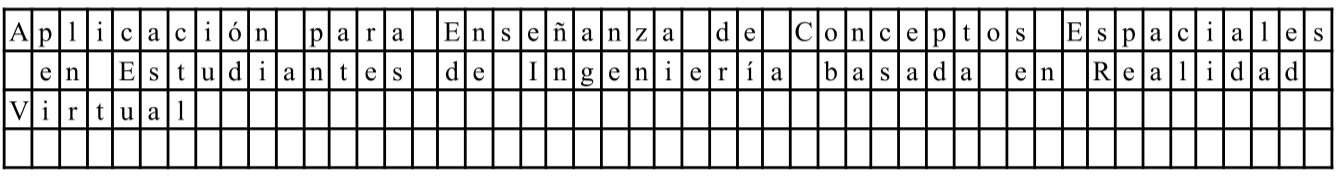
\includegraphics[width=\textwidth]{nombre-04-24.png}
\end{figure}

\subsection*{Datos del Estudiante:}
\begin{table}[h]
  \doublespacing
  \begin{tabularx}{\textwidth}{X c c c}
    \hline
    \textbf{Apellidos, Nombres} & \textbf{C.I.N.}    & \textbf{Teléfono} & \textbf{e-mail}  \\
    \hline
    \small{\estudiante}         & \small{28.031.941} & \small{Insertar}  & \small{Insertar} \\
    \hline
  \end{tabularx}
\end{table}

\subsection*{Datos del Tutor Académico:}

\begin{table}[h]
  \onehalfspacing
  \begin{tabularx}{\textwidth}{>{\hsize=.3\hsize}X X}
    Nombre                       & \academicTutor                                                                       \\
    C.I.N.                       & Insertar                                                                             \\
    Profesión                    & Insertar                                                                             \\
    Años Experiencia Profesional & Insertar                                                                             \\
    Cargo Actual                 & Insertar                                                                             \\
    E-mail                       & Insertar                                                                             \\
    Teléfonos                    & Insertar \tab Oficina: Insertar                                                      \\
    \hline
    Años de Graduado             &
    Insertar \tab[4cm] Tutor TG \hfill Sí \space\fbox{$\checkmark$} \hfill No \space\fbox{\phantom{a}}                  \\
    \hline
    Profesor UCAB                & Sí \space\fbox{$\checkmark$} No \space\fbox{\phantom{a}} \tab[2cm] Escuela: Insertar \\
  \end{tabularx}
\end{table}

\clearpage

\section*{Historial de Revisiones}

\begin{table}[h]
  \begin{tabularx}{\textwidth}{>{\raggedright\arraybackslash\hsize=.5\hsize}X X}
    \textbf{Nombre Estudiante}                        & \estudiante \\
    \textbf{Título del Trabajo Experimental de Grado} & \titulo     \\
  \end{tabularx}
\end{table}

\newcolumntype{E}{>{\centering\arraybackslash\hsize=\hsize}X}
\newcolumntype{T}{>{\raggedright\arraybackslash}m{6cm}}

\begin{table}[h]
  \doublespacing
  \begin{tabularx}{\textwidth}{|E|T|T|}
    \hline
    \textbf{Fecha} & \centering\arraybackslash\textbf{Razón del Rechazo}                                                                                                                                       & \centering\arraybackslash\textbf{Modificación Realizada} \\
    \hline
    26/04/2025     & Se solicitan ajustes en el título de la propuesta, alcance, limitaciones y antecedentes, corrección de uso del título, cambios de forma con respecto a las viñetas y tabla de cronograma. & Ajustes según las indicaciones dadas.                    \\
    \hline
    28/04/2025     & Se solicitan ajustes en el alcance y limitaciones, revisión en la redacción de justificación y cambio de forma en el indice.                                                              & Ajustes según las indicaciones dadas.                    \\
    \hline
  \end{tabularx}
\end{table}

\clearpage


\thispagestyle{empty}
\tableofcontents
\clearpage

\pagestyle{plain}
\pagenumbering{arabic}
\setcounter{page}{1}
% TODO - Interconectar parrafos para mayor fluidez de lectura

\usection{Planteamiento del Problema}
% Qué es la Visión Espacial? (Concepto)
La visión espacial, o visualización, es definida por \citeauthor{piaget1971} \citeyear{piaget1971} como la capacidad de las personas para generar representaciones mentales del espacio. Estas actúan como guías que permiten entender y trabajar con el espacio, ya sea al dibujar un plano o al resolver un problema de geometría. De manera similar \citeauthor{sanjuan2016vision} \citeyear{sanjuan2016vision} define la visión espacial como la habilidad de operar mentalmente con imágenes visuales o espaciales.

% Utilidad e importancia
De acuerdo con \citeauthor{wai2009spatial} \citeyear{wai2009spatial} la importancia de la visión espacial reside en su capacidad para mejorar la comprensión y manipulación del espacio. Esto resulta vital en campos como la arquitectura, el diseño, la ingeniería y las artes visuales. Además, esta habilidad está estrechamente relacionada con el éxito en áreas de ciencias, tecnología, ingeniería y matemáticas (CTIM), como lo demuestran los estudios revisados por \citeauthor{wai2009spatial} \citeyear{wai2009spatial}, que indican que las habilidades espaciales predicen el rendimiento académico en estas disciplinas. Por lo tanto, desarrollar y mejorar la visión espacial no solo beneficia el rendimiento profesional, sino también el desarrollo cognitivo y la resolución de problemas en general.

% Desafios en la enseñanza de conceptos espaciales
% Como se enseña tradicionalmente
% Qué pasa? (Evidencias)
% Por qué pasa? (Causas)
El estudio de \citeauthor{ramos2025ensenanza} \citeyear{ramos2025ensenanza} identifica varios desafíos en la enseñanza de conceptos espaciales en la educación básica. Los resultados muestran una dificultad entre los estudiantes para identificar objetos en el aula y se observa que las actividades de enseñanza no siempre se perciben como claras o contextualmente aplicables. El estudio también destaca una inconsistencia en la frecuencia de las actividades relacionadas con el espacio y un uso irregular de recursos didácticos como mapas y modelos tridimensionales. Se identifica una subutilización de aplicaciones tecnológicas en la enseñanza de estos conceptos. Estos hallazgos indican áreas de mejora en los enfoques educativos actuales para la enseñanza de conceptos espaciales.

% Qué pasa si no se hace nada? (Tendencias)
La literatura, como evidencian \citeauthor{gunderson2012relation} \citeyear{gunderson2012relation} y \citeauthor{hawes2020explains} \citeyear{hawes2020explains}, establece una clara relación entre las habilidades espaciales, el desarrollo cognitivo general y la capacidad para abordar problemas complejos. Se destaca también que el subdesarrollo de estas habilidades podría comprometer significativamente la capacidad de los estudiantes para adaptarse a entornos cambiantes y complejos, así como su rendimiento académico y desarrollo profesional.

% Qué se puede hacer? (Solucion propuesta)
Ante los desafíos identificados y la importancia de las habilidades espaciales, se propone el desarrollo de una aplicación para la enseñanza de conceptos espaciales en estudiantes de ingeniería basada en realidad virtual. Esta aplicación buscará superar las limitaciones de los métodos tradicionales, ofreciendo una experiencia inmersiva e interactiva. Su diseño se centrará en la intuitividad y facilidad de uso, permitiendo a los estudiantes explorar y manipular conceptos espaciales de manera práctica y atractiva. La realidad virtual ofrece la posibilidad de crear entornos tridimensionales simulados que facilitan la comprensión de conceptos abstractos, permitiendo a los estudiantes experimentar y aplicar sus conocimientos en un contexto virtual realista.

\clearpage

\usection{Objetivos}

\usubsection{Objetivo General}
Desarrollar una aplicación para enseñanza de conceptos espaciales en estudiantes de ingeniería basada en realidad virtual.


\usubsection{Objetivos Específicos}

\newcommand{\oeOne}{Analizar la situacion que presentan los estudiantes de ingenieria al abordar conceptos espaciales, identificando las necesidades y requerimientos para el desarrollo de la aplicación.}
\newcommand{\oeTwo}{Diseñar una aplicación para enseñanza de conceptos espaciales a estudiantes de ingeniería basada en realidad virtual en función del análisis realizado.}
\newcommand{\oeThree}{Implementar la aplicación para enseñanza de conceptos espaciales a estudiantes de ingeniería basada en realidad virtual según el diseño realizado.}
\newcommand{\oeFour}{Validar la aplicación para enseñanza de conceptos espaciales a estudiantes de ingeniería basada en realidad virtual con respecto al análisis realizado}
\newcommand{\oeFive}{Realizar la documentación de la aplicación para enseñanza de conceptos espaciales a estudiantes de ingeniería basada en realidad virtual realizada.}
\begin{enumerate}
  \item \oeOne
  \item \oeTwo
  \item \oeThree
  \item \oeFour
  \item \oeFive
\end{enumerate}

\clearpage

\usection{Alcance}

El presente trabajo se enfocará en el desarrollo de una aplicación basada en realidad virtual para la enseñanza de conceptos espaciales, orientada a fortalecer la visión espacial en estudiantes de ingeniería. La aplicación estará dirigida a estudiantes que cursen asignaturas relacionadas con conceptos matemáticos y geométricos, y se desarrollará utilizando tecnologías de Realidad Virtual Inmersiva, haciendo uso de dispositivos Meta Quest. El desarrollo se llevará a cabo en la Universidad Católica Andrés Bello en un plazo de 20 semanas, teniendo en cuenta lo siguiente:

\begin{itemize}
  \item Se realizará un análisis y levantamiento de requerimientos para identificar las necesidades de los usuarios y definir las funcionalidades a implementar en la aplicación.
  \item Se diseñará la arquitectura de la aplicación, definiendo los componentes y su interacción, así como la interfaz de usuario.
  \item Se implementará la aplicación utilizando el motor gráfico Unity, haciendo uso de un dispositivo de realidad virtual Meta Quest, integrando los modelos 3D y las funcionalidades definidas en la fase de diseño.
  \item Se hará una validación de la aplicación con usuarios reales, recolectando feedback para realizar mejoras y ajustes necesarios.
  \item Se realizará una documentación de la aplicación, incluyendo el manual de usuario y la guía de instalación.
        % NOTE
        % \item El producto final permitirá a los usuarios interactuar con objetos tridimensionales en un entorno virtual inmersivo, facilitando la comprensión de conceptos espaciales, aplicando:
        %       \begin{itemize}
        %         \item Interfaces de usuario intuitivas.
        %         \item Diagramado de ecuaciones escritas por el usuario.
        %         \item Libertad de movimiento por el entorno virtual generado.
        %         \item Herramientas de manipulación de los objetos generados.
        %         \item Parametrización de los objetos.
        %         \item Visualización de puntos de intersección.
        %         \item Uso de deslizadores para la visualización de ecuaciones en distintos estados cuando la variable toma un valor dado.
        %         \item Representación de vectores y magnitudes en el espacio.
        %         \item Representación de campos vectoriales y escalares en el espacio.
        %       \end{itemize}
\end{itemize}

\clearpage

\usection{Limitaciones}

\lipsum[1-2]

\clearpage

\usection{Justificación}
La presente investigación se motiva en la necesidad continua de mejora en los métodos de enseñanza de la ingeniería, particularmente en el desarrollo de la visión espacial, una habilidad crucial para el éxito profesional en este campo. El desarrollo de un entorno de enseñanza basado en realidad virtual (RV) ofrecerá una solución efectiva para superar las limitaciones de los métodos tradicionales.

\begin{itemize}
  \item La visión espacial es un pilar fundamental para la comprensión y aplicación de conceptos complejos dentro del campo de la ingeniería, abarcando el diseño, la construcción y el análisis de estructuras y sistemas. Sin embargo, los métodos de enseñanza tradicionales, que a menudo se basan en representaciones bidimensionales y modelos físicos estáticos, pueden limitar el desarrollo de una comprensión profunda de los conceptos espaciales por parte de los estudiantes. En consecuencia, se observa una brecha significativa entre las habilidades espaciales que demanda el entorno laboral y las que los estudiantes adquieren a través de la educación convencional.
  \item El proyecto aportaría la creación de entornos de enseñanza inmersivos e interactivos mediante realidad virtual para facilitar la visualización y manipulación tridimensional de objetos y conceptos, permitiendo simular escenarios complejos y abstractos de forma práctica y segura, y promoviendo una enseñanza intuitiva y significativa con retroalimentación inmediata.
  \item Los beneficiarios directos serán los estudiantes de ingeniería, quienes mejorarían significativamente su visión espacial para un mayor rendimiento académico y mejor preparación profesional; mientras que los beneficiarios indirectos incluirían las instituciones educativas, que podrían modernizar su enseñanza y atraer talento, y el sector industrial, que se beneficiaría de ingenieros con habilidades espaciales avanzadas, impulsando la innovación y la competitividad.
  \item Alineación con los Objetivos de Desarrollo Sostenible ODS 4, Educación de Calidad (Meta 4.4): El proyecto contribuiría a garantizar una educación inclusiva y equitativa de calidad, y a promover oportunidades de enseñanza permanente para todos.
  \item El proyecto sentaría las bases para futuras investigaciones y desarrollos en educación de ingeniería y afines mediante tecnologías inmersivas como la realidad virtual, permitiendo la creación de un modelo de enseñanza replicable y escalable a otras instituciones y áreas, contribuyendo así a una cultura de innovación y la adopción de tecnologías emergentes para mejorar la calidad educativa.
\end{itemize}

\clearpage

\usection{Marco Referencial}

\usubsection{Antecedentes}
\subsubsection*{Insert [Insertar]}
\lipsum[1-2]


\usubsection{Bases Teóricas}
\lipsum[2]

% TODO - Desarrollar Bases teoricas
\usubsubsection{Insertar}

\lipsum[1-2]


\clearpage

\usection{Procedimiento Metodológico}

\lipsum[2]

\usubsection{Justificación de la Metodología}

\lipsum[3]

\clearpage

% Descripción detallada de la planificación del proyecto. Por cada objetivo específico: descripción de tareas a realizar para alcanzarlo, destacando producto y su distribución en el tiempo; aquí se definen actividades y entregables a medida que el proyecto avanza; ver Anexo A2 – Ejemplo Referencial de Cronograma de Actividades
\usection{Cronograma de Trabajo}

% Color Column
\newcommand{\cc}{\cellcolor[HTML]{4bacc6}}
\newcolumntype{L}{>{\raggedright\arraybackslash\hsize=.435\hsize}X}
\newcolumntype{S}{>{\centering\arraybackslash\hsize=.045\hsize}X}

\newcommand{\tableObjective}[2]{
  \vspace{-2em}
  \begin{table}[!ht]
    \begin{tabularx}{\textwidth}{|X|}
      \hline
      \textbf{#1.} #2 \\
      \hline
    \end{tabularx}
  \end{table}
  \FloatBarrier
  \vspace{-2em}
}

\newcommand{\workScheduleHeader}{
  \begin{table}[!ht]
    \onehalfspacing
    \hfill
    \begin{tabularx}{0.63\textwidth}{|X|}
      \hline
      \centering\arraybackslash\textbf{Bloque Semanal (2 Semanas / Bloque)} \\
      \hline
    \end{tabularx}
  \end{table}
  \vspace{-2em}
  \begin{table}[!ht]
    \onehalfspacing
    \begin{tabularx}{\textwidth}{|L|S|S|S|S|S|S|S|S|S|S|}
      \hline
      \centering\arraybackslash\textbf{Actividades por Objetivo} & \textbf{1} & \textbf{2} & \textbf{3} & \textbf{4} & \textbf{5} & \textbf{6} & \textbf{7} & \textbf{8} & \textbf{9} & \textbf{10} \\
      \hline
    \end{tabularx}
  \end{table}
}

\workScheduleHeader
\tableObjective{1}{\oeOne}
\begin{table}[!ht]
  \begin{tabularx}{\textwidth}{|L|S|S|S|S|S|S|S|S|S|S|}
    \hline
    Analizar la situación que presentan los estudiantes de ingeniería al abordar conceptos espaciales para identificar necesidades y requerimientos generales en la aplicación. & \cc & \cc &     &  &  &  &  &  &  & \\
    \hline
    Definir los requerimientos funcionales y no funcionales de la aplicación a desarrollar con respecto al análisis general hecho anteriormente.                                &     &     & \cc &  &  &  &  &  &  & \\
    \hline
  \end{tabularx}
\end{table}
\tableObjective{2}{\oeTwo}
\begin{table}[!ht]
  \begin{tabularx}{\textwidth}{|L|S|S|S|S|S|S|S|S|S|S|}
    \hline
    Diseñar la arquitectura y la interfaz de usuario de la aplicación. &  &  & \cc & \cc &  &  &  &  &  & \\
    \hline
    Diseñar la lógica y funcionalidad de la aplicación.                &  &  & \cc & \cc &  &  &  &  &  & \\
    \hline
    Diseñar protocolo de pruebas.                                      &  &  & \cc & \cc &  &  &  &  &  & \\
    \hline
  \end{tabularx}
\end{table}

\tableObjective{3}{\oeThree}
\begin{table}[!ht]
  \begin{tabularx}{\textwidth}{|L|S|S|S|S|S|S|S|S|S|S|}
    \hline
    Implementar módulos definidos, de acuerdo al diseño realizado. &  &  &  &  & \cc & \cc & \cc & \cc &  & \\
    \hline
    Aplicar protocolo de pruebas diseñado.                         &  &  &  &  & \cc & \cc & \cc & \cc &  & \\
    \hline
    Realizar ajustes de acuerdo a pruebas realizadas.              &  &  &  &  & \cc & \cc & \cc & \cc &  & \\
    \hline
  \end{tabularx}
\end{table}
\clearpage
\workScheduleHeader
\tableObjective{4}{\oeFour}
\begin{table}[!ht]
  \begin{tabularx}{\textwidth}{|L|S|S|S|S|S|S|S|S|S|S|}
    \hline
    Realizar pruebas y validación con usuarios.           &  &  &  &  &  &  &  &  & \cc & \\
    \hline
    Realizar ajustes de acuerdo a validación de usuarios. &  &  &  &  &  &  &  &  & \cc & \\
    \hline
  \end{tabularx}
\end{table}
\tableObjective{5}{\oeFive}
\begin{table}[ht!]
  \begin{tabularx}{\textwidth}{|L|S|S|S|S|S|S|S|S|S|S|}
    \hline
    Realizar documentación técnica.    &  &  &  &  &  &  & \cc & \cc & \cc & \cc \\
    \hline
    Realizar documentación de usuario. &  &  &  &  &  &  &     &     & \cc & \cc \\
    \hline
  \end{tabularx}
\end{table}

\clearpage

\phantomsection
\bibliography{references}

\end{document}
